\chapter{实验与分析}
%通过对分层存储优化领域相关成果的研究学习,总结了如下结论:
%\begin{compactitem}
%    \item 在文件系统中,文件或数据块之间的静态关联广泛存在,只与文件系统结构有关,不受应用运行状态影响。反过来,这种静态关联一定程度上影响着应用运行时数据访问的规律。
%    \item 可采用频繁序列挖掘算法,N-gram模型及循环神经网络等序列分析手段来分析应用的数据访问规律。
%\end{compactitem}

%在第三章理论模型的阐述中,我们提出了三条假设:
%
%1.POSIX文件系统下,构成路径的文件名和目录名满足分布式语义假设。根据该假设,我们采用词嵌入方法将文件名和目录名映射为向量,以表达它们存在的上下文关系。
%
%2.在假设1成立的前提下,采用词嵌入方法将文件名或目录名映射为向量后,将各级词向量线性相加得到的路径向量,可以表达文件之间的静态关联。
%
%3.在假设1、2成立的前提下,路径向量不受应用运行状态的影响。相反地,路径向量所蕴含的静态关联可以帮助分析应用运行时的数据访问规律。根据该假设,我们将路径向量作为循环神经网络的输入建立模型,用以分析应用的数据访问规律。本文涉及的具体任务是解决文件的冷热分类问题。
%
%本实验以验证以上假设和相关模型合理性为主要目的。
本章主要对本课题中提出的三条假设以及建立的相关模型进行验证实验和结果分析。首先介绍本课题的工作负载选择和数据采集方法等实验准备工作,然后介绍实验设计与评估指标,最后分析实验结果,验证模型有效性。

\section{实验设计与性能指标}
编译是计算机应用中最常见的工作负载之一,具有以下特点:文件和目录命名规范,语义明确;运行过程固定,文件访问顺序由Makefile和其他配置文件唯一决定,访问模式单一且可重复;小文件众多,不属于缓存友好的负载。

基于以上特点,我们认为编译任务比较适合选为初期实验的工作负载。本实验中,我们选取GlusterFS、Ceph、Lustre、openAFS和NFS-ganesha等5个开源文件系统项目作为实验对象。

本实验以模型验证为主,因此采用单机环境配置,具体配置如下:处理器2.2 GHz Intel Core i7,内存8GB 1600 MHz DDR3;GlusterFS配置为trace-posix的单机双层模块,其中trace层的作用是对工作负载的文件访问请求进行追踪与记录。


%\begin{table}[htbp]
%\centering
%\begin{minipage}[t]{0.9\linewidth}
%\caption{实验环境设置}
%\label{tab:experiment_env}
%\begin{tabularx}{\linewidth}{cZcZc}
%\toprule[1.5pt]
%    &   {\hei 参数} &   {\hei 配置}\\
%\hline
%\multirow{3}*{硬件环境}    &   处理器  &  Intel Core i7 4核 2.2 GHz \\
%\cline{2-3}
%    &   内存    &   8GB 1600MHz DDR3 \\
%    &   硬盘    &   500GB 75MB/s    \\
%\hline
%软件环境    &   操作系统    &   CentOS7 Linux内核3.10\\
%            &   文件系统    &   GlusterFS   \\
%\bottomrule[1.5pt]
%\end{tabularx}
%\end{minipage}
%\end{table}                                                                                             




\subsection{词嵌入模型实验}
\begin{table}[htbp]
\centering
\begin{minipage}[t]{0.9\linewidth}
\caption{词嵌入模型数据集}
\label{tab:samples}
\begin{tabularx}{\linewidth}{cZcZ}
\toprule[1.5pt]
{\hei 项目名称} & {\hei 项目大小(MB)} & {\hei 生成路径样本数}\\
\midrule[1pt]
GlusterFS& 137.5 & 3277\\
Ceph& 524.6 & 11893\\
Lustre& 232.8 & 2045\\
openAFS& 207.6 & 6144\\
nfs-ganesha& 123.5 & 992\\
合计& 1226.0 & 24351\\
\bottomrule[1.5pt]
\end{tabularx}
\end{minipage}
\end{table}

为了构造词嵌入模型实验的数据集(语料库),本实验将上述5个开源项目源代码存放于同一目录/test下,然后以/test为根节点遍历整个文件目录,将所有结点对应的路径写入数据集文本文件,每一条路径样本相当于自然语言处理中的一个句子样本。表\ref{tab:samples}分别列出了5个子目录生成的样本数,共计24351条。该实验的主要工作是利用Skip-gram算法训练上述数据集,并将最终形成的词向量进行PCA降维与可视化。

\subsection{冷热文件分类实验}
在该实验中,本研究在GlusterFS中实现了一个简易的trace模块,其功能是在工作负载运行过程中追踪所有的文件打开操作(trace\_open),将要打开的文件路径参数导出到数据集,并通过训练好的词嵌入模型将每条文件路径转化为路径向量。为了测试模型对单进程与多进程负载的效果,我们分别采用了两种方式生成数据集。第一种是依次编译5个工程生成训练集,然后打乱编译执行顺序生成测试集;第二种是开启多进程对5个工程同时编译(各个进程开始的时间随机,但尽量保证较长的重合时段)的方式,生成训练集和测试集,以模拟多进程同时访问文件系统的场景。
%模型测试的评价指标,按照实际应用需求主要分为两个场景:

%第一种场景是缓存容量充足时,需要尽可能地将热数据迁入到缓存中,目的是避免遗漏,从而提高缓存命中率,此时最重要的指标是精确率(Precision)
二分类模型的评价指标主要包括精确率(Precision),召回率(Recall),假正例率(FPR)和真正例率(TPR)。设分类阈值为$\alpha$,这四项指标可解释如下:

\begin{equation}
    P = \frac{TP}{TP + FP}
\end{equation}
为精确率,其含义为分类正确的正样本个数占所有被分为正样本个数的比例,也就是分类成热数据中的确是热数据的比例。%缓存容量充足时,需要尽可能地将热数据迁入到缓存中,目的是避免遗漏,从而提高缓存命中率,此时精确率越高越好,可以适当降低阈值$\alpha$。

%第二种场景是缓存不足时,需要尽可能避免将冷数据误判为热数据,此时主要考虑的指标是召回率(Recall)
\begin{equation}
    R = \frac{TP}{TP + FN}
\end{equation}
表示召回率,即热数据被正确识别的比例。%当缓存容量不足,数据缓存操作需要避免冷数据误判为热数据时,召回率越高越好,此时宜提高分类阈值。

以上两项指标随分类阈值变化而变化,阈值从0到1变化产生的所有精确率-召回率的二元组画成的图称为P-R图。性能优异的模型,能在图上找到一个合适的阈值,使得两项指标都比较高。
%精确率和召回率通常难以兼得,性能优异的分类器可以找到一个最佳阈值,使得精确率和召回率都保持在较好的水平;反过来,性能不佳的分类器则会发生如下情况:调低阈值时召回率迅速降低,缓存空间会很快被无用的冷数据挤占,上调阈值则会导致精确率迅速下降,尽管
\begin{equation}
    FPR = \frac{FP}{TN+FP}
\end{equation}
表示假正例率,即冷数据被误判为热数据的比例。该项数据越低越好。

\begin{equation}
    TPR = \frac{TP}{TP+FN}
\end{equation}
表示真正例率,与召回率同义。

在模型固定的情况下,FPR与TPR同样随分类阈值$\alpha$的调整而变化,FPR-TPR二元组所作的图称为ROC曲线。区别模型优劣的关键在于,能否找到一个最优的阈值,使得FPR较低的情况下仍能维持较高的TPR。
%在模型所有参数固定的情况下,直接决定以上指标的是分类阈值,该阈值与模型性能无关,只与场景需求有关,可随GLusterFS的设置动态适配。通常情况下精确率与召回率是此消彼长的,性能优异的模型应当尽量兼顾两者。我们将采用P-R曲线,ROC曲线和AUC值作为评价标准。

\section{实验结果与分析}

\subsection{路径嵌入}
路径嵌入模型训练完毕后,生成的词汇表大小为1322。图\ref{fig:experiments/PCA_15_1}为词汇表作降维处理后,出现频率最高的15个词的可视化结果。
\begin{figure}[htp]
\centering
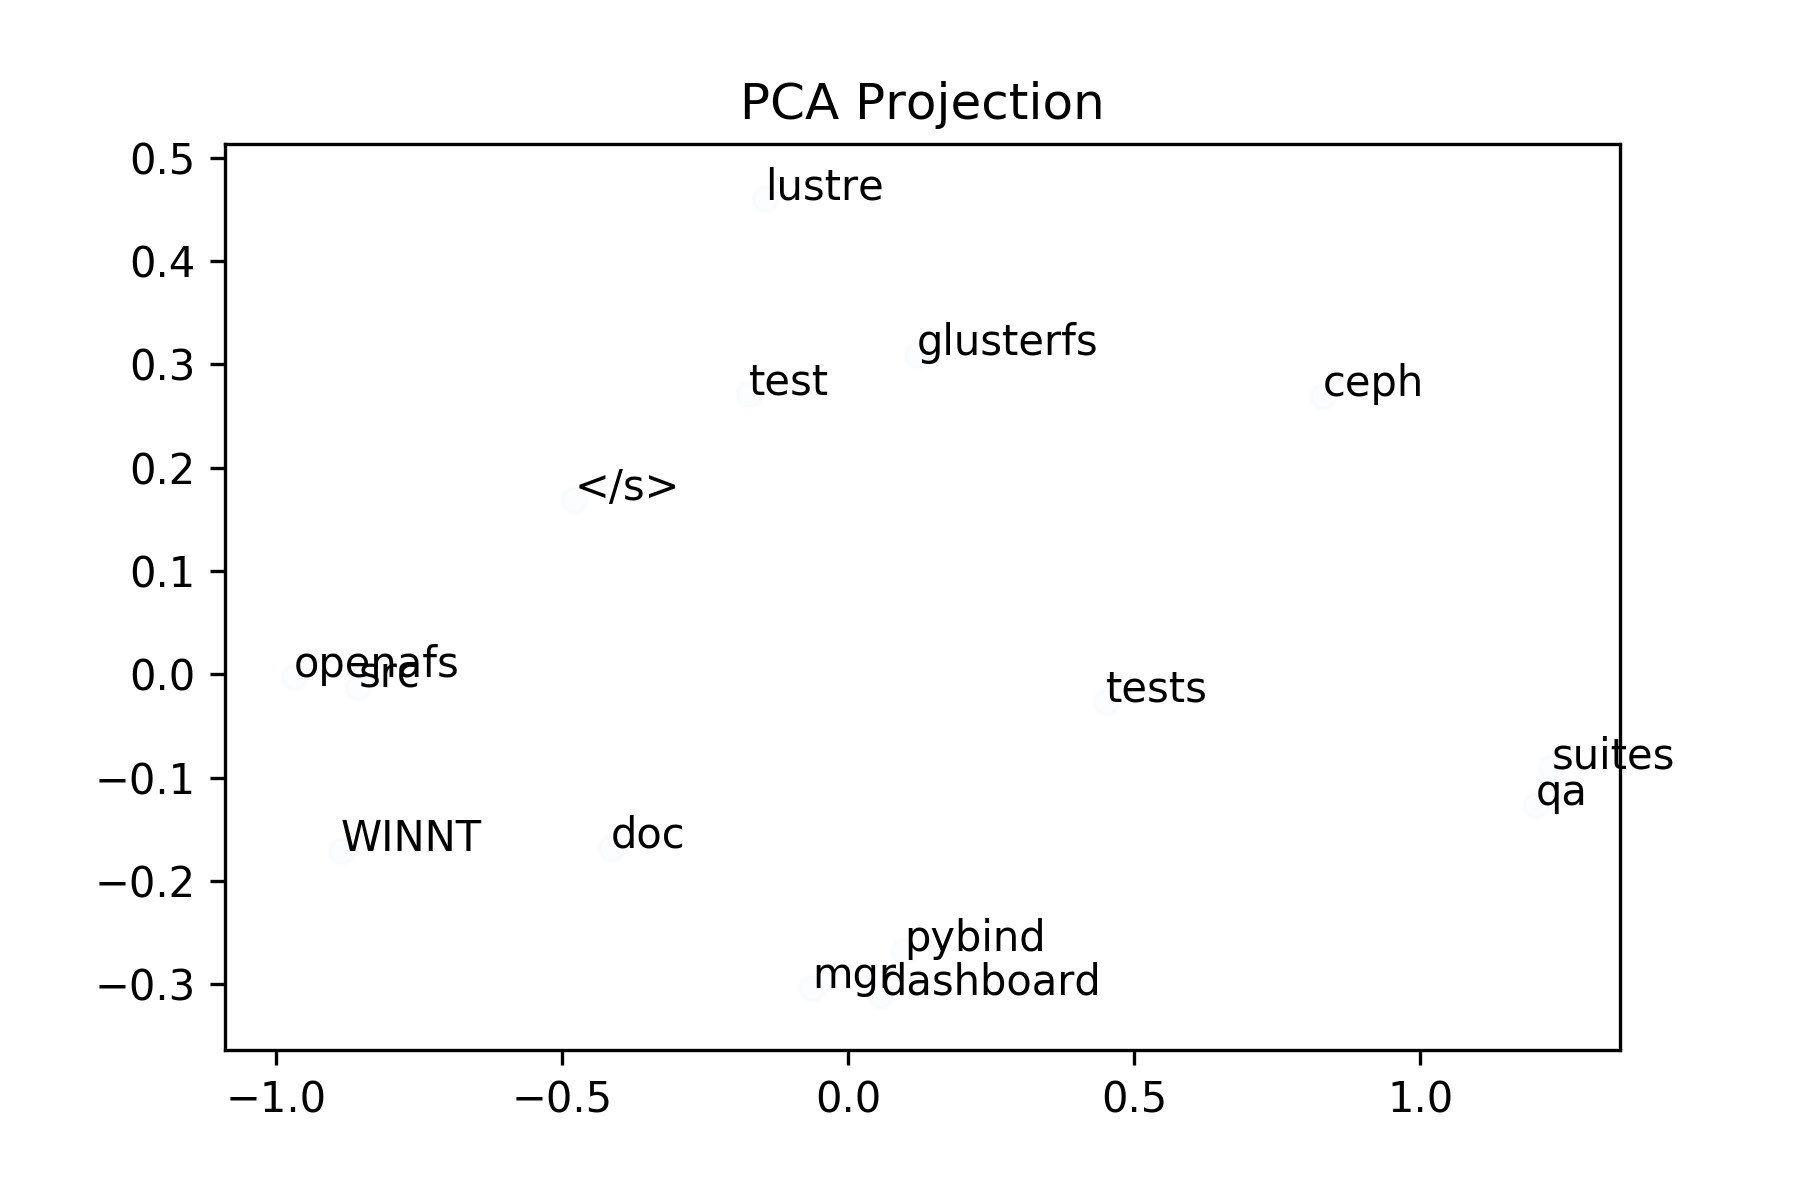
\includegraphics[width=\textwidth]{experiments/PCA_15_1}
\caption{15个最高频率词}
\label{fig:experiments/PCA_15_1}
\end{figure}




\subsection{冷热文件分类}


\begin{figure}[htp]
\centering
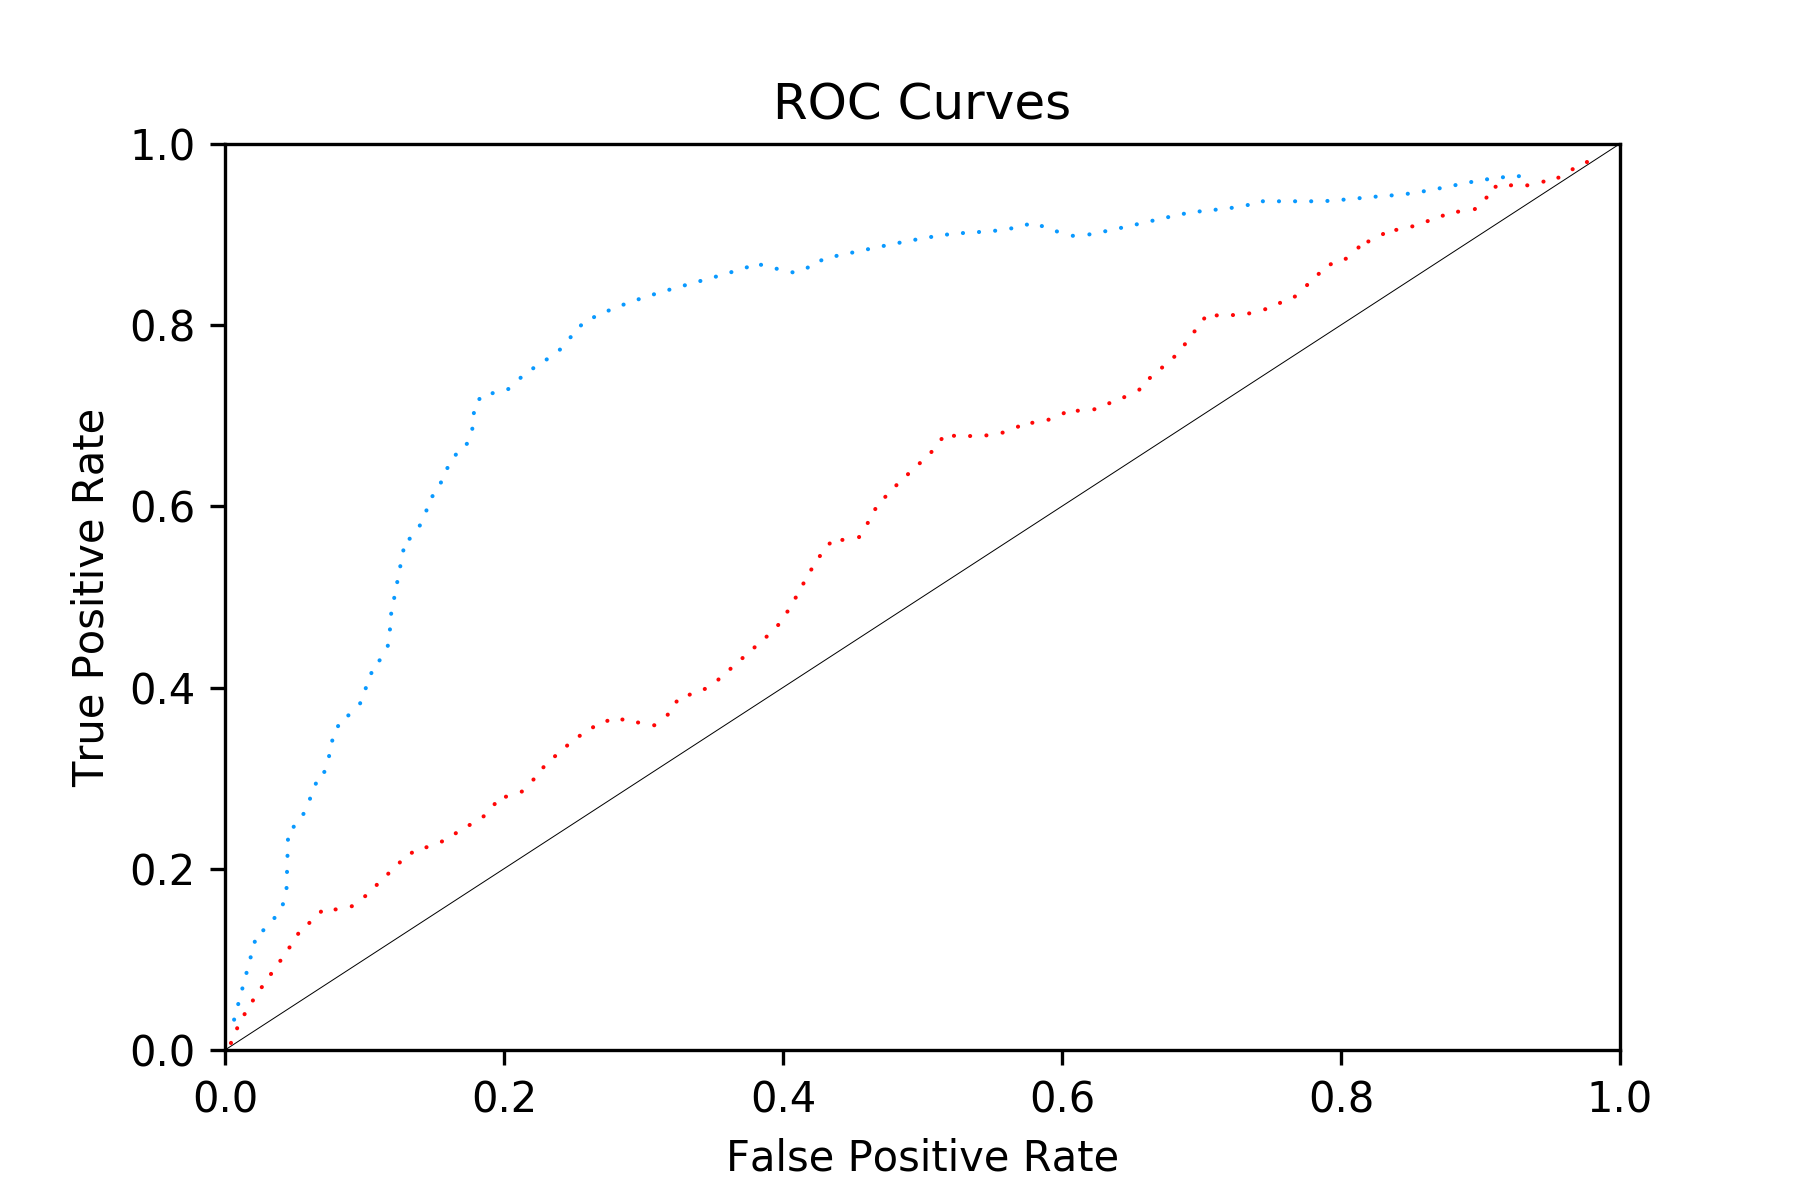
\includegraphics[width=\textwidth]{experiments/ROC}
\caption{ROC曲线}
\label{fig:ROC}
\end{figure}

图\ref{fig:ROC}为ROC曲线,蓝色点迹为单进程编译任务下的模型表现。可以看出,该模型性能尚可,实验结果中存在一个较优阈值$\alpha$=0.43时,热数据被发现识别的比例达到80\%以上,且冷数据被误判为热数据的概率控制在25\%;相对的,该模型在多进程编译任务中的数据分类性能很差,热数据识别率与冷数据误判率几乎同步,意味着其效果相当于随机缓存策略。

图\ref{fig:PR}为P-R曲线。在该指标下,模型在单进程任务中的表现略好于多进程任务,但整体性能一般,无法找到某个阈值使得精确率与召回率均达到令人满意的水平。

\begin{figure}[htp]
\centering
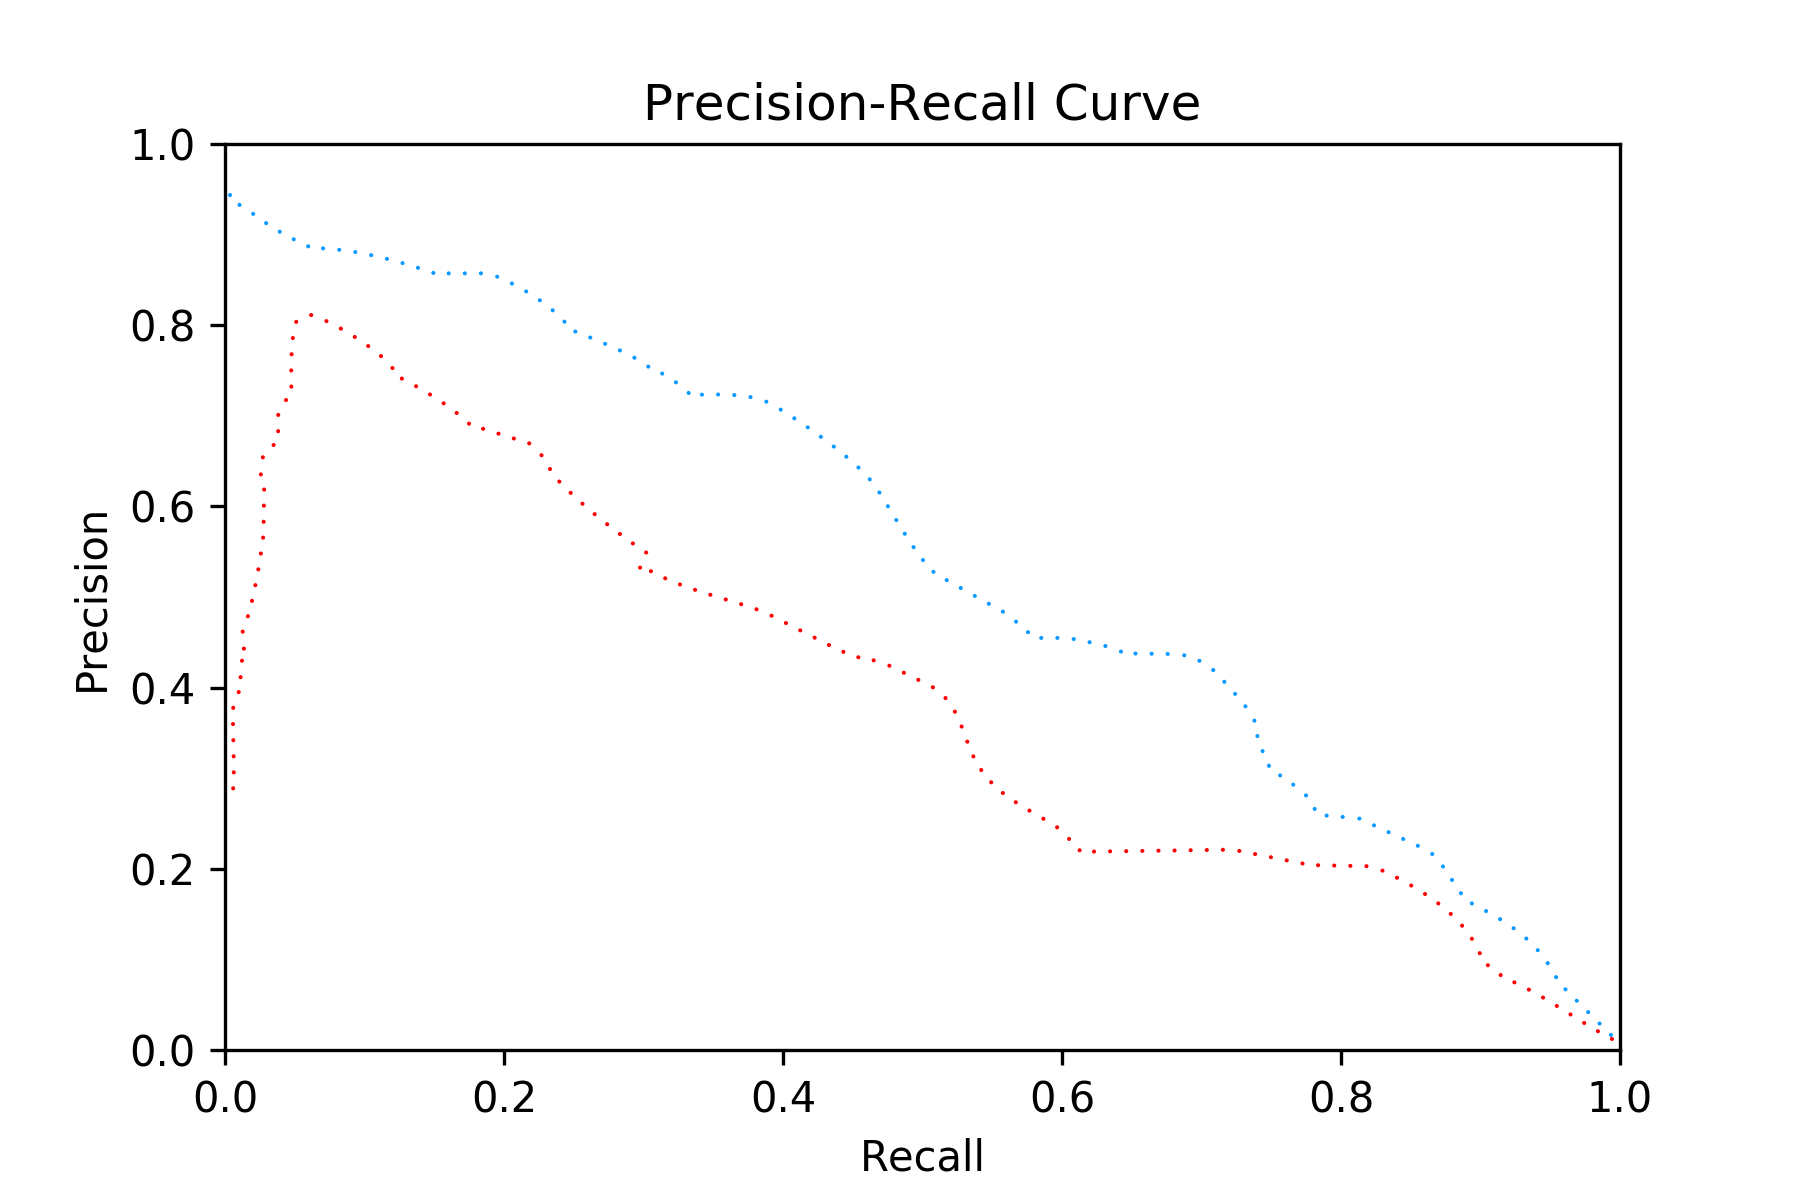
\includegraphics[width=\textwidth]{experiments/PR}
\caption{PR曲线}
\label{fig:PR}
\end{figure}

\section{本章小结}
本章以编译任务为工作负载设计了两项实验,分别是路径嵌入模型试验和基于门控神经网络的热点数据识别实验。实验结果表明,该模型在单进程任务上取得了一定的效果,但对多进程任务运行时热点数据的识别性能较弱。